\section{Methodology}
% \begin{figure*}[h]
%     \centering
%     \includegraphics[trim={0cm 5.1cm 0cm 0cm}, clip, width=0.9\linewidth]{figures/NOCTA-Figures.pdf}
%     \caption{An overview of \texttt{\OurMethod}. The framework starts at time $t$ with observed features $x_o$ and a set of $|\mathcal{O}|$ binary candidate masks $v$ of size $M\times (L - t)$, indicating plans of future features to acquire from time $t + 1$ to $L$. \texttt{\OurMethod} provides two complementary estimators (\texttt{\OurMethod-NP} and \texttt{\OurMethod-P})
%     to predict the accuracy-cost tradeoff for each plan. 
%     After selecting the optimal plan, \texttt{\OurMethod} predicts for the time points up to the next scheduled visit $t_{\text{next}}$, and acquires the corresponding features $x_{t_{\text{next}}}$, which are appended to $x_o$. After acquiring this new data, the entire process repeats and moves to the immediate next time step $t_{\text{next}} > t$. This allows \texttt{\OurMethod} to dynamically reassess and revise its acquisition plan based on the most recent information rather than being locked into a static plan.
% }    
%     % It then selects the mask with the minimum estimated tradeoff value, predicts for the time points up to the next scheduled visit $t_{\text{next}}$, and acquires the corresponding features $x_{t_{\text{next}}}$, which are appended to $x_o$. This estimation-prediction-acquisition-reassessment cycle is repeated at each subsequent timestep $t_{\text{next}} > t$ until the final timestep $L$ is reached.}
%     % % process repeats at the next time step $t_{\text{next}} > t$ until the final time step $L$ is reached.}
%     \label{fig:lafa_v2}
% \end{figure*}

% \begin{figure*}[h]
%     \centering
%     \includegraphics[trim={0cm 2.7cm 0cm 0cm}, clip, width=0.99\linewidth]{figures/overview.pdf}
%     \caption{An overview of the \texttt{\OurMethod} framework. Starting at time step $t$ with the observed features $x_o$ and a set of candidate acquisition masks, \texttt{\OurMethod} provides two complementary estimators (\texttt{\OurMethod-NP} and \texttt{\OurMethod-P})
%     to predict the accuracy–cost tradeoff for each candidate. 
%     It then selects the mask with the minimum estimated tradeoff value, predicts for the time points up to the next scheduled visit, and acquires the corresponding features $x_v$, which are appended to $x_o$. This process repeats at the next time step $t' > t$ until the final time step T is reached.}
%     \label{fig:lafa}
% \end{figure*}


% \textbf{Notation.}\quad We formally define the longitudinal AFA setup: let $\mathcal{D} = \{(x_i, y_i)\}_{i=1}^N$ denote the dataset of $N$ instances (e.g., patients). For each $i$, $x_i$ is a temporal sequence with $L$ time steps, i.e., $x_i = \{x_{i,t}\}_{t=1}^L$, with $t \in \{1, \ldots, L\}$ indexing the time step. At each time step, $x_{i,t} \in \mathbb{R}^M$ includes measurements of $M$ (costly) features (note that it is possible to extend to individual acquisitions that yield multi-dimensional feature vectors for multi-modal cases). %i.e., $x_{i,t}=\{x^m_{i,t} \in \mathbb{R}^{d_m} \}_{m=1}^M$. %Note that it is possible for $x^m_{i,t} = \emptyset$, which indicates the feature is unobserved.  
% In this work, we focus on a classification task where labels $y_{i,t} \in \{1, 2, \ldots, C\}$ are defined for each timepoint $t$, and $C$ represents the number of classes. Following \citet{qin2024risk, yoon2019asac}, each feature $m$ has a time-invariant  \footnote{\texttt{\OurMethod} easily extends to time-varying costs by replacing $c^m$ with $c^{m, t}$ (cost of modality $m$ at time $t$).} cost $c^m$. Lastly, we use colons to represent selecting subsequences along a specific axis; for example, $x_{1:t} = (x_1, \ldots, x_t)$ represents the measurements from timepoint $1$ to $t$.
\textbf{Notation}\quad We consider longitudinal AFA over a dataset $\mathcal{D} = \{(x_i, y_i)\}_{i=1}^N$ of $N$ instances (e.g., patients). For each instance $i$, the covariates form a sequence of length $L$: $x_i = \{x_{i,t}\}_{t=1}^L$, where $t \in \{1, \ldots, L\}$ indexes the time step. At each time step $t$, $x_{i,t} \in \mathbb{R}^M$ contains $M$ (costly) feature measurements, but the policy may only acquire a subset at each visit \footnote{\texttt{\OurMethod} also supports multi-modal acquisitions where each modality yields a vector; this can be modeled by replacing scalar features with modality-specific vectors.}. We study a classification task with per-timepoint labels $y_{i,t} \in \{1, 2, \ldots, C\}$, where $C$ represents the number of classes. Following \citet{qin2024risk, yoon2019asac}, each feature $m$ has a time-invariant\footnote{\texttt{\OurMethod} easily extends to time-varying costs by replacing $c^m$ with $c^{m, t}$ (cost of modality $m$ at time $t$).} cost $c^m$. Finally, we use colon notation for subsequences; for example, $x_{1:t} = (x_1, \ldots, x_t)$ denotes measurements from timepoints $1$ to $t$ (inclusive).


% \subsection{Why is Longitudinal AFA MDP a Challenging Problem?}
\subsection{Longitudinal AFA modeled as an MDP}

% Longitudinal AFA modeled as an MDP}

Longitudinal AFA can be formulated as a Markov Decision Process (MDP). The state $s_t = \bigl({x}_{o},\, o,\,  t\bigr)$, where ${x}_{o}$ denotes the (partial) observations before time $t$ and $o \subseteq \{(m, t') \mid m \in \{1, \ldots, M\}, \, t' \in \{1, \ldots,  t-1\}\}$ records which features were acquired. 
We suppose access to a pre-trained arbitrary conditioning classifier $\hat{y}$ ~\citep{shim2018joint, li2021active} that can predict the label at any target timepoint $k$ with the current information, i.e., $\hat{y}_k(x_o)$. Note that the same input information can be used to predict at other time points, $\hat{y}_{k^\prime}(x_o)$ (where forward prediction corresponds to when feature observations in $o$ occur before $k^\prime$).
The action space is $a \in \{a_{t'}\}_{t'=t}^L \cup \{\varnothing\}$, where $a_{t'} \in \{0,1\}^M$ indicates which of the $M$ features to acquire at time $t'$, or, when $a = \varnothing$, to terminate and predict all remaining timepoints. For a non-terminal action, the transition is $\bigl({x}_{o},\, o, \, t\bigr) \rightarrow \bigl({x}_{o \cup a_{t'}},\, o \cup a_{t'},\, t'+1 \bigr)$, where (for notational simplicity) $o \cup a_{t'}$ denotes the union of the previous acquisitions and tuples of features at time $t'$ in $a_{t'}$.
Since this implies that we are not acquiring any information until time $t'$, the reward is the negative cross-entropy (CE) loss of making predictions up to $t'$ (i.e., $\hat{y}_{t}, \ldots, \hat{y}_{t'-1}$) with previous information (${x}_{o}$) and respective negative CE loss and cost of acquiring new features at time $t'$: 
$-\sum_{k=t}^{t'-1} \mathrm{CE}(\hat{y}_k({x}_{o}),\,y_{k}\bigr) - \mathrm{CE}(\hat{y}_{t'}({x}_{o \cup a_{t'}}),\,y_{t'}\bigr) -\alpha\sum_{m=1}^M a_{t',m}c^m$, 
where $\alpha$ is an \emph{application-specific} accuracy-cost tradeoff parameter; certain applications allow a higher cost (i.e., lower $\alpha$) and some are more cost-restricted (i.e., high $\alpha$). When terminated ($a = \varnothing$) at timepoint $t$, we are not acquiring any additional information for the remaining timepoints, thus the reward is $-\sum_{k=t}^L \mathrm{CE}(\hat{y}_k({x}_{o}),\,y_{k}\bigr)$, which represents the negative cross-entropy loss accumulated from $t$ to $L$ using the current information at hand.
We denote our policy as $\pi\bigl({x}_{o},\, o,\, t\bigr)$, which selects 
actions to maximize the expected cumulative rewards through $L$.\looseness-1


\textbf{Longitudinal AFA MDP Challenges}\quad Modeling longitudinal AFA as an MDP introduces several difficulties: (1) \emph{a large and complicated action space}, since one requires decisions on when to acquire and which features to acquire; (2) \emph{a complicated state space}, as it evolves dynamically over the combinatorial acquisitions as new features are captured over time; and (3) \emph{a credit assignment problem}, since acquisitions are awarded at an aggregate level, it is hard to disentangle exactly which of the acquired features were most responsible for prediction rewards \citep{li2021active}.
Despite these challenges, prior work \citep{qin2024risk, yoon2019asac, kossen2022active, nguyen2024active} often relies on RL for longitudinal AFA. In contrast, we propose \texttt{\OurMethod}, an RL-free approach that not only provides a theoretical lower bound on the optimal longitudinal AFA MDP value (see Appx.~\ref{appendex:theorem}), but also empirically outperforms RL-based baselines. \looseness-1


\subsection{Non-Greedy Objective Cost-Tradeoff}


We now introduce \texttt{\OurMethod} through a novel  longitudinal objective that provides a provable (see below) proxy for the MDP value of states. Let $\mathcal{V}_{>t} = {\{(m, t') \mid m \in \{1, \ldots, M\}, \, t' \in \{t+1, \ldots, L\}\}}$ represent the set of candidate feature-time pairs that are still available to acquire after time $t$. At a partially observed state $(x_o, o, t)$, we have two options: (1) \emph{choose an acquisition plan} $v \subseteq  \mathcal{V}_{>t}$ (which specifies what to acquire in the future), or (2) \emph{terminate acquisition} (i.e., $v = \varnothing$) and make predictions for the remaining timepoints using only the currently observed information $x_o$.
% we ask: (1) \emph{which subset in $\mathcal{V}$ should we acquire} to balance the tradeoff between improved accuracy and acquisition cost, or (2) \emph{should we terminate and make the prediction} for the remaining time points based on what we have observed in $x_o$? 
The \textbf{n}on-greedy \textbf{o}bjective \textbf{c}ost-\textbf{t}radeoff (NOCT) determines the tradeoff of an acquisition plan of additional features $v \subseteq  \mathcal{V}_{>t}$ for a current partially known instance of $x_o$ ($o$ containing features from the past, $\leq t$):
% \setlength{\abovedisplayskip}{5pt}
% \setlength{\belowdisplayskip}{5pt}
% \begin{equation}
% u\bigl({x}_{o}, o\bigr)  \! =  \! 
% \underset{v \subseteq  \mathcal{V}}{\arg\!\min}\, \mathbb{E}_{y_{t+1:L}, x_v \mid {x}_{o}}[\ell (x_o \cup x_v, y, t)] + \alpha \!\!\!\!\! \sum_{(m, t') \in v} \!\!\!\! c^m,
% \label{eq:obj}
% \end{equation}
% \begin{equation}
% \resizebox{\linewidth}{!}{%
% $
% \mathrm{NOCT}\bigl({x}_{o}, o, v\bigr)  \! =  \! 
% \mathbb{E}_{y_{t+1:L}, x_v \mid {x}_{o}}[\ell (x_o \cup x_v, y, t)] + \alpha \! \sum_{(m, t') \in v} \! c^m
% $
% },
% \label{eq:obj}
% \end{equation}
\begin{align}
&\mathrm{NOCT}\bigl({x}_{o}, o, v\bigr)   \equiv  \nonumber \\ 
&\quad\quad \mathbb{E}_{y_{t+1:L}, x_v \mid {x}_{o}}[\ell (x_o \cup x_v, y, t)] + \alpha \!\!\! \sum_{(m, t') \in v} \!\!\! c^m,\label{eq:obj} %\\
% &\mathrm{where} \nonumber \\ 
% &\ell (x_o \cup x_v, y, t) \equiv \sum_{k=t+1}^L \mathrm{CE}\bigl(\hat{y}_k({x}_{o} \cup {x}_{v_{t+1:k}}),\,y_{k}\bigr) 
% \label{eq:pred_loss}
\end{align}

% where 
% \begin{equation}
% \ell (x_o \cup x_v, y, t) = \sum_{k=t+1}^L \mathrm{CE}\bigl(\hat{y}_k({x}_{o} \cup {x}_{v_{t+1:k}}),\,y_{k}\bigr),
% \label{eq:pred_loss}
% \end{equation}
% represents the accumulated loss when only acquiring the set of future feature-time pairs in the plan $v$, and ${x}_{v_{t+1:k}}$ denotes the features in the candidate subset $v$ from time step $t+1$ to time step $k$; i.e., $\ell$ captures the quality of predictions, using the temporally available feature according to the plan $v$, which rely on what will be current and previously captured data. 

where $\ell (x_o \cup x_v, y, t) \equiv \sum_{k=t+1}^L \mathrm{CE}\bigl(\hat{y}_k({x}_{o} \cup {x}_{v_{t+1:k}}),\,y_{k}\bigr) $ is the accumulated cross-entropy loss from $t{+}1$ to $L$ when acquiring the future feature-time pairs specified by $v$. 
Here, $x_{v_{t+1:k}}$ denotes the subset of acquired features in $v$ whose time indices lie in $\{t{+}1,\ldots,k\}$, i.e., the features that would be available by time $k$ under plan $v$, given the currently observed information $x_o$. Using trajectories $(x_v, y_{t+1:L})$ in the training set $\mathcal{D}$, the expectation in Eq.~(\ref{eq:obj}) can be directly estimated within an instance during training. At inference time, $x_v$ is unobserved, so we approximate Eq.~(\ref{eq:obj}) using the estimator in Sec.~\ref{subsec:nonparam} and Sec.~\ref{subsec:param}. Intuitively, Eq.~(\ref{eq:obj}) looks ahead at how acquiring a new set of feature-time pairs in $\mathcal{V}_{>t}$ is anticipated to reduce the classification loss from $t+1$ to $L$, while penalizing the acquisition cost (see Fig.~\ref{fig:noct}(a)). For simplicity, we refer to feature-time pairs as ``features''.  %in the remainder of the paper.

% \setlength{\abovedisplayskip}{5pt}
% \setlength{\belowdisplayskip}{5pt}
% \begin{equation}
% \begin{split}
% u\bigl({x}_{o}, o\bigr) = 
% &\underset{v \subseteq  V \cup \{\varnothing\}}{\arg \min } \mathbb{E}_{y_{t:L}, x_v \mid {x}_{o}}[\ell (x_o \cup x_v, y, t)] + \alpha \sum_{a \in v} c^a,
% \end{split}
% \label{eq:obj}
% \end{equation}
% where 
% % {\small
% \begin{equation}
% \ell (x_o \cup x_v, y, t) = \frac{1}{L-t+1}\sum_{k=t}^L \mathrm{CE}(\hat{y}({x}_{o}, {x}_{v_{1:k}}),\,y_{k}\bigr)
% \end{equation}
% represents the accumulated 
% loss when acquiring the set of future features $v$. Intuitively, eq. (\ref{eq:obj}) looks ahead at how acquiring a new set of features in $V$ might reduce the classification loss from time $t$ to $L$, while penalizing the cost of obtaining new features. 


\begin{figure*}[t]
    \centering
    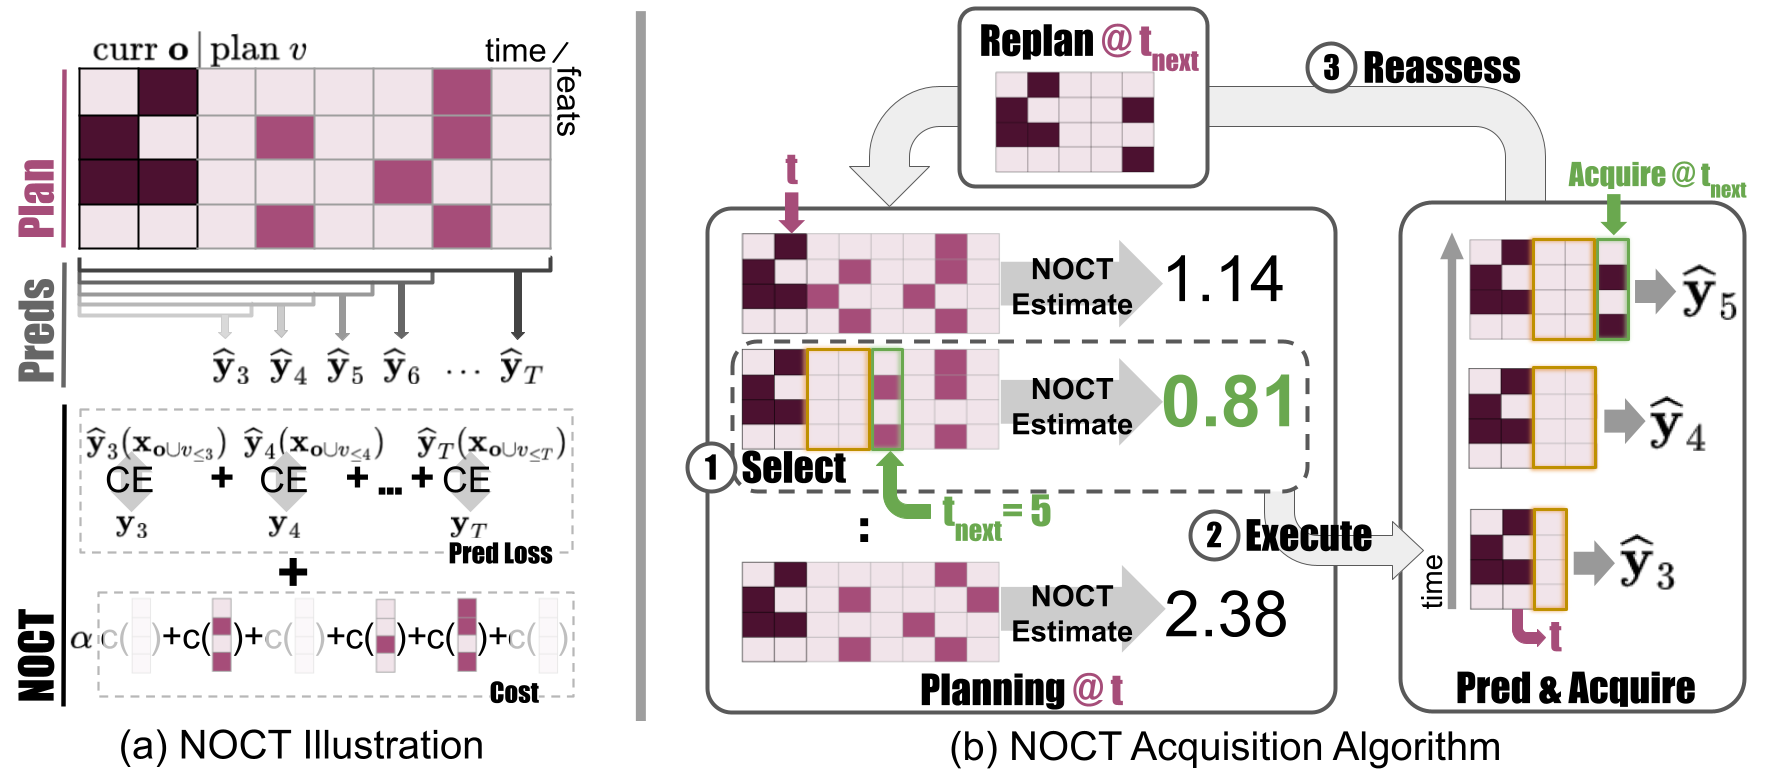
\includegraphics[trim={0cm 0cm 0cm 0cm}, clip, width=0.825\textwidth]{figures/NOCTA_highlevel.png}
    \caption{Overview of \texttt{\OurMethod}. \textbf{(a) NOCT evaluation of plan.}  Given partially observed state $(x_o, o, t)$, a candidate plan $v \subseteq \mathcal{V}_{>t}$ (a feature$\times$time matrix) is evaluated by the tradeoff of (i) the expected accumulated predictive cross-entropy (CE) loss for future acquisitions from $t+1$ to $L$ and (ii) the acquisition cost of selected future acquisitions (i.e., $\alpha \sum_{(m, t') \in v} c^m$). Under plan $v$, the prediction at future time $k$ only uses acquisitions up to time $k$ (i.e., $\hat{y}_{k}(x_{o\cup v_{\le k}})$).
    \textbf{(b) Acquisition algorithm.} At state $(x_o, o, t)$, the \texttt{NOCTA} algorithm evaluates candidate plans $v \subseteq \mathcal{V}_{>t}$ with a NOCT estimator. (1) We \emph{select} the best plan, $\hat{u}$, according to the NOCT estimates. (2) We \emph{execute} the selected plan up to its next acquisition (i.e., $t_{\text{next}}\equiv\min{t':(m,t')\in \hat{u}}$) by acquiring $a_{t_{\text{next}}} \equiv \{(m,t_{\text{next}})\in \hat{u}\}$. Predictions are made at every timepoint; e.g., as illustrated, with $t=2$ and $t_{\text{next}}=5$, \texttt{\OurMethod} predicts at $t=3, 4$ using current information (i.e., $\hat{y}_{3}(x_o), \hat{y}_{4}(x_o))$ and predicts at $t_{\text{next}}=5$ using newly observed features (i.e., $\hat{y}_{5}(x_{o\cup a_{t_{\text{next}}}})$). (3) We \emph{reassess} with $x_o \equiv x_{o\cup a_{t_{\text{next}}}}$ and $t \equiv t_\text{next}$, repeating until the selected plan is empty ($\hat{u}=\varnothing$) or when we reach the final time step ($t= L$). 
    }
    \label{fig:noct}
\end{figure*}

\subsection{NOCT Acquisition (\OurMethod)}

At time $t$, one may use NOCT (Eq.~(\ref{eq:obj})) to indicate the best anticipated future acquisition plan given the current information, $u\bigl(x_o, o\bigr)$:
\begin{equation}
u\bigl({x}_{o}, o\bigr)  \equiv  
\underset{v \subseteq  \mathcal{V}_{>t}}{\arg\!\min}\, \mathrm{NOCT}({x}_{o}, o, v);
\label{eq:nocta}
\end{equation}
i.e., plan according to the anticipated cost tradeoff of obtaining future features for future prediction targets. In fact, we can show that the \texttt{NOCTA} criterion in Eq.~(\ref{eq:nocta}) is a principled proxy value for partially acquired states:
\begin{theorem}
\label{thm:lowerbound}
(Informal) $-\mathrm{NOCT}$ lower bounds the value of the optimal longitudinal AFA MDP policy
\end{theorem}
% \textbf{Theorem 3.1.} \emph{(Informal) The NOCT objective \todo{Dzung: Changed to NOCT} lower bounds the value of the optimal longitudinal AFA MDP policy}.

In other words, acquiring by following the plan selected in Eq.~(\ref{eq:nocta}) serves as an approximation to the optimal longitudinal AFA MDP policy (full proof in Appx.~\ref{appendex:theorem}).




\textbf{Acquisition Algorithm}\quad When Eq.~(\ref{eq:nocta}) returns $u\bigl(x_o, o\bigr) = \varnothing$, it indicates that the potential loss improvement does not justify the cost of acquiring further future features, so we stop acquiring and predict for all subsequent time points using the currently observed features $x_o$. Otherwise, if a non-empty plan $u\bigl(x_o, o\bigr) = v \subseteq \mathcal{V}_{>t}$ is selected, it indicates that, given $x_o$, the set $u\bigl(x_o, o\bigr)$ yields the best trade-off for future predictions. Carrying out the selected plan $u\bigl(x_o, o\bigr)$, implies that the next acquisition occurs at $t_{\text{next} } \equiv \min\{\,t'\mid(m,t')\in u(x_o,o)\}$, the earliest timepoint in the plan. This implies that all the predictions until $t_{\text{next} }$ are to be done with the current information, $\hat{y}_{t+1}({x}_{o}), \ldots, \hat{y}_{t_{\text{next}}-1}({x}_{o})$, and the prediction at $t_{\text{next}}$ includes the planned features at $t_{\text{next}}$, $a_{t_{\text{next}}} \equiv \{(m,t_{\text{next}})\mid(m,t_{\text{next}})\in u(x_o,o)\}$, $\hat{y}_{t_{\text{next}}}({x}_{o \cup a_{t_{\text{next}}}})$. We may similarly continue with acquisitions in $u\bigl(x_o, o\bigr)$ for timepoints after $t_{\text{next}}$. However, a more dynamic strategy is to incorporate the newly acquired feature values to reassess (update) the best anticipated plan. That is, compute $u\bigl({x}_{o \cup a_{t_{\text{next}}}}, o \cup a_{t_{\text{next}}}\bigr)$ using $\mathcal{V}_{t_{\text{next}}}$, for further acquisitions after $t_{\text{next}}$ (see Fig.~\ref{fig:noct}(b)). 



% \textbf{Proposition 3.2.} \emph{(Informal) Replanning after each acquisition is never worse (in $\mathrm{NOCT}$ value) than committing to the original plan’s remainder (full proof in Appx. \ref{appendex:proposition1}).}
\begin{proposition}
\label{prop:replanning}
(Informal) Replanning after each acquisition is never worse (in terms of the $\mathrm{NOCT}$ objective) than committing to the original plan’s remainder (full proof in Appx.~\ref{appendex:proposition1}).
\end{proposition}


Note that $u\bigl({x}_{o \cup a_{t_{\text{next}}}}, o \cup a_{t_{\text{next}}}\bigr)$ is a dominating strategy to simply proceeding with $u\bigl(x_o, o\bigr)$ since: 1) it incorporates additional information, which provides more context (using values in $a_{t_{\text{next}}}$) for the anticipated utility of further acquisitions; 2) the search for $u\bigl({x}_{o \cup a_{t_{\text{next}}}}, o \cup a_{t_{\text{next}}}\bigr)$ includes the original plan for further acquisition from $u\bigl(x_o, o\bigr)$, so it may stick to the previous plan if it is still anticipated to be optimal in light of new values. Intuitively, this dynamic strategy avoids a stubborn approach that does not update its acquisition plans in light of additional information. The acquisition process of \texttt{\OurMethod} is detailed in Alg.~\ref{alg:nocta}.

\begin{algorithm}[htp]
    \footnotesize
  \caption{\texttt{\OurMethod} \label{alg:nocta}}
  \begin{algorithmic}[1]
    \Require Number of features $M$, number of time steps $L$, cost for feature $m$ as $c^m$, estimator $\hat y_{k}$.

    \State Initialize: \texttt{predictions} $\gets [\,]$; \texttt{terminate} $\gets$ \texttt{false}; $t \gets 0$; $o \gets \varnothing$
    
    % \State Initialize \texttt{terminate} $\gets$ \texttt{false}
    % \State Initialize $t \gets 1$
    \While{not \texttt{terminate}}
    \State $\mathcal{V}_{>t} \! \gets\!  \{(m,t') \! \mid \! m\in\{1,\ldots,M\},\,t'\in\{t+1,\ldots,L\}\}$
      \State $\hat u(x_o,o)\approx
    \underset{v \subseteq  \mathcal{V}_{>t}} {\arg\!\min}\,\mathrm{NOCT}(x_o, o, v)$ \Comment{Approx.}
      \If{$\hat u(x_o,o)=\varnothing$}
        \State $t_{\text{next} }\gets L$; \texttt{terminate} $\gets$ 
        \texttt{true}
      \Else
        \State $t_{\text{next}}\gets\min\{\,t'\mid(m,t')\in\hat u(x_o,o)\}$
        \State $o\gets o\cup\{(m,t_{\text{next}})\mid(m,t_{\text{next}})\in\hat u(x_o,o)\}$
      \EndIf
        \For{$t' = t+1,\dots,t_{\text{next}}$}
          \State append $\hat{y} _{t'}\bigl(x_{o_{1:t'}}\bigr)$ to \texttt{predictions}
        \EndFor
        \State $t \gets t_{\text{next}}$
%
    \EndWhile
    \State \Return \texttt{predictions}
  \end{algorithmic}
\end{algorithm}

Note that NOCT (Eq.~(\ref{eq:obj})) is not directly tractable at inference time, since it requires knowledge of the ground-truth conditionals $y_{t+1:L}, x_v \mid {x}_{o}$; thus, we proceed with estimate of NOCT and $u(x_o, o)$, which we develop below. 
% \textbf{Proposition 2} \emph{(Informal) If $\widehat{\mathrm{NOCT}}$ estimates $\mathrm{NOCT}$ within $\varepsilon$ error at each replanning round, then the resulting policy is at most $O(s\varepsilon)$ worse than oracle-\texttt{\OurMethod}, where $s$ is the maximum number of remaining acquisition rounds (proof in Appx. \ref{appendex:regret}).}

% In other words, this implies that a small error in $\widehat{\mathrm{NOCT}}$ cannot cause a large degradation in the overall sequential decision plan, and the bound degrades only linearly with the number of acquisition rounds $s$.

% are acquired, the model predicts for the subsequent time points until the next scheduled acquisitions. 
% This non-greedy policy for \texttt{\OurMethod} 
% %is \emph{simpler to estimate than a full MDP solution, yet still 
% directly balances the tradeoff between acquisition cost and predictive performance. 

%  The acquisition process of \texttt{\OurMethod} is detailed in Algorithm~\ref{alg:nocta}. Intuitively, \texttt{\OurMethod} mirrors the clinical workflow: order tests, read results, and reassess. When \texttt{\OurMethod} selects the acquisition plan $\hat u(x_o,o)$, we do not commit to the entire sequence. Instead, we only execute the acquisition scheduled at the immediate next time point $t_{\text{next}}$, update the observed features $(x_o,o)$, and replan the acquisition schedule. Note that the model can also continue on with its original plan if it still believes those remaining acquisitions are optimal in light of the new acquired information in $t_\text{next}$. This iterative design reflects the principle that as new observed features alter our belief about the labels, it should also update our estimate of the utility of yet-to-be-acquired information.




 % However, evaluating this objective is intractable as in practice we do not have access to the true expectation of labels and unacquired values for the test samples, $\mathbb{E}_{y_{t+1:L}, x_v \mid {x}_{o}}$ in Eq. (\ref{eq:obj}). We therefore develop two ways to estimate $u\bigl({x}_{o}, o\bigr)$: a non-parametric method that uses nearest neighbors on learned embedding space (Sec. \ref{subsec:nonparam}) and a parametric method that directly predicts the accuracy-cost tradeoff (Sec. \ref{subsec:param}). 

% Following \cite{valancius2023acquisition}, one may connect our \texttt{\OurMethod} acquisition objective (Eq. (\ref{alg:nocta})) to the full RL optimization via a lower bound.
% % In other words, the optimal longitudinal AFA MDP policy is guaranteed to perform no worse than \texttt{NOCTA}. A proof of this result can be found in Appendix \ref{appendex:theorem}.
% In other words, acquiring according to the \texttt{NOCTA} objective (Eq. (\ref{eq:obj})) serves as an approximation to the optimum longitudinal AFA MDP. Additional details can be found in Appendix \ref{appendex:theorem}.

% Following \cite{valancius2023acquisition}, one may connect our \texttt{\OurMethod} acquisition objective (Eq. (\ref{alg:nocta})) to the full RL optimization via a lower bound:

% To connect our \texttt{\OurMethod} acquisition objective (Eq. (\ref{alg:nocta})) to the full RL optimization, we cast both problems to maximization and have the following guarantee:

% \textbf{Theorem 1.} \emph{The value of the optimal longitudinal AFA MDP policy is lower bounded by \texttt{\OurMethod}}.

% % In other words, the optimal longitudinal AFA MDP policy is guaranteed to perform no worse than \texttt{NOCTA}. A proof of this result can be found in Appendix \ref{appendex:theorem}.
% In other words, acquiring according to the \texttt{NOCTA} objective (Eq. (\ref{eq:obj})) serves as an approximation to the optimum longitudinal AFA MDP. A proof of this result can be found in Appendix \ref{appendex:theorem}.

% \begin{algorithm}[tb]
%   \caption{\texttt{\OurMethod}: Non‑Greedy Optimal Cost–Tradeoff Acquisition}
%   \label{alg:nocta}
%   \begin{algorithmic}[1]
%     \Require Observed features $o$ (possibly $o=\varnothing$), instance values $x_{o}$, \\
%              \quad\;\;number of features $M$, number of timesteps $L$, \\
%              \quad\;\;costs $c^{a}$ for each feature $a$, trade‑off $\alpha>0$, estimator $f_{k}$
%     \Ensure A sequence of intermediate predictions \texttt{predictions}
%     \State \textbf{initialize} \texttt{terminate} $\gets$ \texttt{false}
%     \State \textbf{initialize} \texttt{predictions} $\gets [\,]$
%     \State \textbf{initialize} $t \gets 1$
%     \While{$t \le L$ \textbf{and} not \texttt{terminate}}
%       \State $V \gets \{(m,t') \mid m\in\{1,\dots,M\},\,t'\in\{t,\dots,L\}\}\setminus o$
%       \State $\hat u \;\gets\;\displaystyle
%         \underset{v\subseteq V}{\arg\min}\Bigl[
%           \E_{y_{t:L},x_v\mid x_o}\,\ell(x_o\cup x_v,y,t)
%           \;+\;\alpha\sum_{a\in v}c^a
%         \Bigr]$
%       \If{$\hat u = \varnothing$}
%         \State \texttt{terminate} $\gets$ \texttt{true}
%       \Else
%         \State $t_{\min}\gets \min\{t'\mid(m,t')\in\hat u\}$
%         \State $o\gets o\;\cup\;\{(m,t_{\min})\mid(m,t_{\min})\in\hat u\}$
%         \For{$i = t,\dots,\min(t_{\min},L)$}
%           \State $\hat y_i \gets f_{k}\bigl(x_{o,1:i}\bigr)$
%           \State append $\hat y_i$ to \texttt{predictions}
%         \EndFor
%         \State $t \gets t_{\min}$
%       \EndIf
%     \EndWhile
%     \State \Return \texttt{predictions}
%   \end{algorithmic}


% \subsection{\texttt{NOCT-Contrastive}}
\subsection{\texttt{NOCT-Contrastive}}
\label{subsec:nonparam}

In this subsection, we introduce \texttt{NOCT-Contrastive}, an embedding-based estimator that enables estimating $\mathrm{NOCT}(x_o,o,v)$ (and therefore $u({x}_{o}, o)$) from partial observations. We train the embedding space with a contrastive loss that embeds instances according to the utility of future acquisitions.

\textbf{Plug-in NOCT}\quad For \emph{training instances}, $(x_i, y_i) \in \mathcal{D}$, the simplest estimate of $\mathrm{NOCT}\bigl({x}_{i,o}, o, v\bigr)$ (Eq.~(\ref{eq:obj})) is a plug-in sample approach:
\begin{equation}
    \scalebox{0.9}{$\displaystyle
        \widehat{\mathrm{NOCT}}_{pl}\bigl({x}_{i,o}, o, v\bigr) =\ell (x_{i,o} \cup x_{i,v}, y_i, t) + \alpha \!\!\! \sum_{(m, t') \in v} \!\!\! c^m.
    $}
    \label{eq:plugobj}
\end{equation}
Note that for a held-out instance, Eq.~(\ref{eq:plugobj}) is not directly computable (it requires future features $x_{i,v}$); we develop inference-time estimators later in this section. For a training instance, we may determine what features are useful when starting from $o$ at time $t$ by ranking candidate future plans $v \subseteq V_{>t}$ using the plug-in objective $\widehat{\mathrm{NOCT}}_{\mathrm{pl}}(x_{i,o},o,v)$ and taking the top-$r$ plans $\hat{v}_{i,o}^{(1)}, \ldots, \hat{v}_{i,o}^{(r)}$ with the smallest values. These top plans induce a future-candidate distribution, $\zeta_{i,o}$, \emph{over future acquisitions} $(m, t')\in V_{>t}$ (and termination $\varnothing$), where $\zeta_{i,o}(m,t')$ is given by a normalized count of how often $(m,t')$ appears in $\hat{v}_{i,o}^{(1)}, \ldots, \hat{v}_{i,o}^{(r)}$. Intuitively, $\zeta_{i,o}$ summarizes which \emph{future} measurements are consistently suggested by the best plans, and we use it in our contrastive loss. The formal $\zeta_{i,o}$ construction in Appx.~\ref{appendex:future_dist}. 

% These top plans induce a future-candidate distribution, $\zeta_{i,o}$, over future acquisitions $(m, t')\in \mathcal{V}_{>t}$  (by a normalized count of occurrences in $\hat{v}_{i,o}^{(1)}, \ldots, \hat{v}_{i,o}^{(r)}$) that we propose to use in a contrastive loss. The formal construction is provided in Appx. ~\ref{appendex:future_dist}
%We construct $\zeta_{i,o}$ as follow: we assign higher weight to plans with lower $\widehat{\mathrm{NOCT}}_{pl}$, count how often each acquisition $(m,t')$ appears among the weighted top-$r$ plans, and normalize the resulting nonnegative scores to sum to $1$. 
% Thus, $\zeta_{i,o}$ is a categorical distribution supported on $\mathcal V_{>t}$ (and $\varnothing$ for termination for empty set $\hat{v}_{i,o}$), where $\zeta_{i,o}(m,t')$ is larger when $(m,t')$ is repeatedly selected by many high-quality plans. Intuitively, $\zeta_{i,o}$ summarizes which future acquisitions are repeatedly favored under the accuracy-cost objective (Eq. (\ref{eq:plugobj})) from the current observed info $x_o$. 

\textbf{Contrastive Learning}\quad We propose to learn an embedding network that maps partially observed features into an embedding space where distances capture the similarity of their acquisition characteristics. Formally, we learn an embedding network $g_\phi(x_{i,o}) \in \mathbb{R}^E$ such that two instances $x_{i,o}$ and $x_{j,o}$ are mapped to nearby points in $\mathbb{R}^E$ if the additional (future) acquisitions available to them are expected to influence their accuracy-cost tradeoff in a similar manner. Conversely, instances with divergent accuracy-cost tradeoff are pushed away in $\mathbb{R}^E$. 

To achieve this, we define a similarity score between instances based on their future-candidate distributions $\zeta_{i, o}$ and $\zeta_{j, o}$, using the exponential of their negative Jensen-Shannon ($\mathrm{JS}$) divergence:
\begin{equation}
      \texttt{sim}_{ij}
    = \exp\!\bigl(-\beta\,\mathrm{JS}(\zeta_{i, o}, \zeta_{j, o})\bigr),
    \label{eq:js}
\end{equation}
where $\beta > 0$ controls how strongly divergence affects similarity. Letting $\delta_{ij} = \bigl\lVert g_\phi \bigl(x_{i,o}\bigr) - g_\phi\bigl(x_{j, o}\bigr)\bigr\rVert^2$ be the embedding distance, we minimize a contrastive loss \citep{chopra2005learning}:
\begin{equation}
\label{eq:ebmedding}
    \scalebox{0.87}{$\displaystyle
    \mathcal{L}_{\mathrm{emb}} = \frac{1}{2} \Bigl(\texttt{sim}_{ij} \cdot \delta_{ij} + 
    (1 - \texttt{sim}_{ij}) \cdot \max \bigl(0,\,\gamma - \delta_{ij}\bigr)^2\Bigr)$},
\end{equation} 
where $\gamma > 0$ is the margin parameter. Minimizing $\mathcal{L}_{\mathrm{emb}}$ encourages $g_\phi$ to create an embedding space where distance reflects the similarity of future-candidate distributions. 

\textbf{\texttt{NOCT-Contrastive}}\quad For held-out instances (at inference time), the plug-in estimate $\widehat{\mathrm{NOCT}}_{pl}$ in Eq.~(\ref{eq:plugobj}) is unavailable because future measurements and labels are unknown. Instead, we approximate $\mathrm{NOCT}(x_o,o,v)$ by aggregating plug-in values from a small retrieved set of training trajectories selected by the learned embedding:
% Instead, we propose to utilize an instance based approach using the proposed embeddings (Eq.~\ref{eq:ebmedding}):
\begin{equation}
\scalebox{0.93}{$\displaystyle \widehat{\mathrm{NOCT}}\bigl({x}_{o}, o, v\bigr)\approx \frac{1}{|\mathcal{I}(x_o)|}\sum_{i \in \mathcal{I}(x_o)} \widehat{\mathrm{NOCT}}_{pl}\bigl({x}_{i,o}, o, v\bigr),$} 
\label{eq:noctanp}
\end{equation}
where $\mathcal{I}(x_o)$ contains the closest training instances induced by $g_\phi$: $d(x_o, x_{i,o}) = \Vert g_\phi{(x_o)} - g_\phi{(x_{i,o})} \Vert_{2}$ (e.g., by distance thresholding or by selecting the top-$K$ most similar instances). Note that since $g_\phi(x_{o})$ embeds instances according to the utility of future acquisition, estimating $\mathrm{NOCT}\bigl({x}_{o}, o, v\bigr)$ in terms of $\widehat{\mathrm{NOCT}}_{pl}\bigl({x}_{i,o}, o, v\bigr)$ for $i\in \mathcal{I}(x_o)$ is a sound, intuitive strategy. Note further that the size of the embedding space is a controllable hyperparameter, enabling efficiency at small dimensionalities. We call this estimator \texttt{NOCT-Contrastive}.

$\widehat{\mathrm{NOCT}}\bigl({x}_{o}, o, v\bigr)$ enables us to estimate $\hat{u}(x_o, o)$ in Alg.~\ref{alg:nocta}, to plan acquisitions at inference time. In practice, instead of an exhaustive search over  $v\subseteq \mathcal{V}_{>t}$, one may consider a distributionally sampled (e.g., uniform random or feature-importance guided) set of candidate plans. 
%of  provides a fast approximation to $\arg\min_{v\subseteq \mathcal{V}^{>t}}\widehat{\mathrm{NOCT}}(x_o,o,v)$ and performs well in our experiments. 
More sophisticated discrete optimizers could be substituted if desired, but typically introduce additional overhead \citep{parker2014discrete, rajeev1992discrete}.

\subsection{\texttt{NOCT-Amortized}}
\label{subsec:param}

%Section~\ref{subsec:nonparam} presented an \emph{instance-based} estimator of $\mathrm{NOCT}(x_o,o,v)$ that averages utilities over training instances in a learned embedding space. 
We now develop \texttt{NOCT-Amortized}, a complementary
approach that amortizes inference and predicts the NOCT value for candidate acquisition plans using a neural network. %We coin this estimator as \texttt{NOCT-Amortized}. 


\textbf{Neural NOCT estimator}\quad We learn an estimator $f_\theta$ that predicts the NOCT value of a candidate plan from \emph{the partial information} $x_o$. Since future features $x_v$ are unknown at inference time, $f_\theta$ is conditioned on
the partial observations $x_o$, a representation of the candidate plan $v$ (e.g., a binary mask over feature-time pairs in $V_{>t}$),
and the current time $t$:
\begin{equation}
f_\theta(x_o, v, t) \;\approx\; \mathrm{NOCT}(x_o,o,v).
\label{eq:noct_direct_pred}
\end{equation}
At inference time, we substitute Eq.~\eqref{eq:noct_direct_pred} into  Alg.~\ref{alg:nocta} and obtain the future candidate plan:
\begin{equation}
\hat u(x_o,o) \;\in\; \arg\min_{v \subseteq V_{>t}} f_\theta(x_o, v, t).
\end{equation}
\paragraph{Training Objective}
During training, we can compute the plug-in target $\widehat{\mathrm{NOCT}}_{pl}(x_o,o,v)$ in Eq.~\eqref{eq:plugobj} because the
ground-truth future values for $x_v$ are available in $\mathcal{D}$. We train $f_\theta$ by minimizing the mean squared error objective:
\begin{align} 
\mathcal{L}_{\mathrm{amort}} ~=~  \big( f_\theta(x_{o}, v, t) - \widehat{\mathrm{NOCT}}_{pl}(x_{o}, o, v) \big)^2. 
\label{eq:value_mse} 
\end{align}
\paragraph{Joint Fine-tuning with the Predictor} To reduce the mismatch between (i) the partially observed inputs used by the predictor $\hat y$ and (ii) the inputs scored by $f_\theta$ during planning, we jointly fine-tune $f_\theta$ and $\hat y$ with
\begin{align}
\mathcal{L}_{\mathrm{joint}}
~=~
\frac{1}{L}\sum_{k=1}^{L} \mathrm{CE}\!\left(\hat y_k(x_{o_{1:k}}), y_k\right)
~+~ \lambda\,\mathcal{L}_{\mathrm{amort}},
\label{eq:direct_joint}
\end{align}
where $\lambda$ trades off predictive accuracy and utility estimation. 

% \todo{Phrase search of plan subsampling as a benefit: many methods could be applied, even simple appraoch works.}

% \todo{JO: what is the major idea??} %In non-parametric setup, once we decide the next desired timepoint, we simultaneously acquire all desired features (for more details, please refer to Alg. \ref{alg:lafanp}).



% Note that applying Eq.~\eqref{eq:prob} to specific training data $(x_i, y_i) \in \mathcal{D}$ having observed feature $o$ will yield its future-candidate distribution $p(\cdot \mid x_{i,o})$.


% two samples $x_i$ and $x_j$ with the same observed feature o is computed as $d(x_{i,o}, x_{j,o}) = \Vert g_\phi (x_{i,o}) - g_\phi(x_{j,o}) \Vert_{2}$.

% We train an embedding network $g_\phi: x_o \mapsto \mathbb{R}^E$ so that two partial observations $x_{i, o}$ and $x_{j,o}$  with similar future distributions $p(\cdot \mid x_{i,o})$ and $p(\cdot \mid x_{j,o})$ lie close in the embedding space, and those with dissimilar distributions lie farther apart. To quantify similarity, we use the exponential of the negative Jensen-Shannon (JS) divergence between these two distributions:
% \begin{equation}
%       \texttt{sim}_{ij}
%     = \exp\!\bigl(-\beta\,\mathrm{JS}(p(\cdot \mid x_{i,o}),\,p(\cdot \mid x_{j,o}))\bigr),
% \end{equation}
% % \end{equation}
% and $\beta>0$ controls how strongly divergence affects similarity. Let 
% \begin{equation}
%       \delta_{ij} = \bigl\lVert g_\phi \bigl(x_{i,o}\bigr) - g_\phi\bigl(x_{j, o}\bigr)\bigr\rVert^2
% \end{equation}
% be the squared distance between embeddings of two partial observations $\bigl(x_{i,o}, x_{j,o}\bigr)$. The embedding loss $\mathcal{L}_{\mathrm{emb}}$ is then defined as a contrastive-type loss \citep{chopra2005learning}:
% {\small
% \begin{equation}
% \label{eq:ebmedding}
%     \mathcal{L}_{\mathrm{emb}} = \frac{1}{2} \Bigl(\texttt{sim}_{ij} \cdot \delta_{ij} + 
%     (1 - \texttt{sim}_{ij}) \cdot \max \bigl(0,\,\gamma - \delta_{ij}\bigr)^2\Bigr),
% \end{equation}
% }where $\gamma>0$ is the margin parameter. Minimizing $\mathcal{L}_{\mathrm{emb}}$ encourages pairs of samples whose future distributions are similar (low JS divergence) to have low Euclidean distance in the embedding space, while pairs with dissimilar distributions (high JS divergence) are pushed apart by a margin. Finally, the distance for two samples $x_i$ and $x_j$ with the same observed feature $o$ is computed as $d\bigl(g_\phi (x_{i,o}), g_\phi(x_{j,o})\bigr)$.


% \subsection{\texttt{\OurMethod-Direct}: Direct Neural Network Estimate}
% \label{subsec:param}

% Section~\ref{sec:noct_est} presented an \emph{instance-based} estimator of $\mathrm{NOCT}(x_o,o,v)$ that averages
% trajectory-level utilities over nearest neighbors in a learned embedding space. We now describe a complementary
% approach that \emph{directly} predicts the NOCT objective for a candidate acquisition plan, avoiding neighbor search at
% test time.

% \todo{Rephrase to be consistent with above. E.g. "instance-based" and use NOCT equations}
% Above, we proposed a non-parametric, neighbor-based approach to estimate our generalized \texttt{\OurMethod} cost objective Eq.~(\ref{eq:obj}). We also develop a direct parametric approach, which estimates the cost objective using a network. We expound on our parametric approach, coined \texttt{\OurMethod-P}, below. 

% \textbf{Estimating $u\bigl({x}_{o}, o\bigr)$.} In order to estimate $u(x_o, o)$ in Eq.~(\ref{eq:obj}) parametrically, we attempt to calculate the utility for all potential subsets $v \subseteq \mathcal{V}$ at current time $t$:
% \begin{equation}
% I_v(x_o, o, t) = \ell (x_o \cup x_v, y, t) + \alpha \!\!\!\! \sum_{(m, t') \in v} \!\!\!\! c^m.
% \label{eq:I}
% \end{equation}
% Since we have access to data during training, this value can be directly calculated for all subsets $v$ for training instances $(x_i, y_i)$. However, this is not the case during evaluation time when $x_v$ becomes unknown. Therefore, we estimate $I_v(x_o, o, t)$ through a value network, which we describe below. 

% \textbf{Value Network.}\quad The value network $f_{\theta}$ predict the utility $I_v(x_o, o, t)$ for all potential subsets. Since future features $x_v$ are unknown during evaluation, the network is only conditioned on observed features $x_o$, a candidate mask $v$, and the current time $t$; and its output is denoted as $f_{\theta}(x_o, v, t)$. Since this output estimates the utility of  $I_v(x_o, o, t)$, we optimize through the mean squared error as:
% \begin{equation}
%     \mathcal{L}_{\mathrm{value}} = \mathrm{MSE}\left(f_{\theta}(x_o, v, t), I_{v}(x_o, o, t)\right)\,.
% \end{equation}
    

% % During inference, the values of the potential subset $x_v$ are not available until we decide to acquire them, hence 
% % To avoid distribution shift during evaluation, we match the distribution of observed subsets $o$ during training to what shall be encountered at inference time. That is, at each acquisition step for both training and inference, we choose the next subset based on $u(x_o, o)=\arg\min_{v \subseteq V} f_\theta(x_o, v, t)$.

% Using this value network, we can estimate Eq.~(\ref{eq:obj}) to derive the future acquisition plan $u\bigl({x}_{o}, o)$.

% To minimize the distribution shift between the features evaluated by the value network and those used by the predictor, we jointly optimize the prediction network $\hat{y}_k$ and the value network $f_{\theta}$ over the candidate subset, resulting in the final loss function as:
% \begin{equation}
%     \mathcal{L}_{\mathrm{\OurMethod\text{-}P}} = \frac{1}{L}\sum_{k=1}^{L}{\mathrm{CE}\bigl(\hat{y}_k({x}_{o_{1:k}}), y_{k}\bigr)} + \lambda \cdot \mathcal{L}_{\mathrm{value}} \,,
%     % \mathcal{L}_{\mathrm{\OurMethod\text{-}P}} = \mathcal{L}_{\mathrm{pred}} + \lambda \cdot \mathcal{L}_{\mathrm{value}} \,,
% \end{equation}
% where $\lambda$ balances the tradeoff between minimizing the prediction error (the cross-entropy loss) and accurately estimating the utility of future acquisitions with the value network ($\mathcal{L}_{\mathrm{value}}$).

% % prediction network loss and the value network loss $\mathcal{L}_{\mathrm{value}}$. 

% % We further describe prediction network and its loss function $\mathcal{L}_{\mathrm{pred}}$ in Sec.~\ref{sec:implementation}.
% % where $\lambda$ balances the prediction network loss $\mathcal{L}_{\mathrm{pred}}$ (e.g., cross-entropy) and the value network loss $\mathcal{L}_{\mathrm{value}}$. We further describe prediction network and its loss function $\mathcal{L}_{\mathrm{pred}}$ in Sec.~\ref{sec:implementation}.